\section{Forest Fire Model}

\begin{frame}{The Forest Fire Cellular Automaton}
  \begin{itemize}
    \item A classic CA model that simulates the spread of fire through a forest.
    \item Each cell is in one of three states:
    \begin{itemize}
      \item \textbf{Empty} (0) --- bare ground
      \item \textbf{Tree} (1) --- living tree
      \item \textbf{Burning} (2) --- tree on fire
    \end{itemize}
    \item The model captures the interplay between \textbf{growth}, \textbf{ignition}, and \textbf{fire spread}.
  \end{itemize}
  \vfill
  \begin{center}
    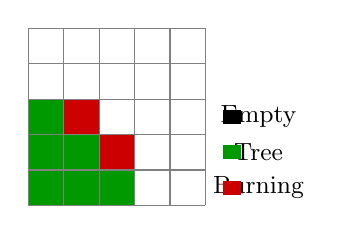
\begin{tikzpicture}[scale=0.45]
      \fill[green!60!black] (0,0) rectangle (1,1);
      \fill[green!60!black] (1,0) rectangle (2,1);
      \fill[green!60!black] (2,0) rectangle (3,1);
      \fill[green!60!black] (0,1) rectangle (1,2);
      \fill[green!60!black] (1,1) rectangle (2,2);
      \fill[red!80!black]   (2,1) rectangle (3,2);
      \fill[green!60!black] (0,2) rectangle (1,3);
      \fill[red!80!black]   (1,2) rectangle (2,3);
      \draw[gray] (0,0) grid (5,5);
      \node at (6.5, 2.5) {\small Empty};
      \node at (6.5, 1.5) {\small Tree};
      \node at (6.5, 0.5) {\small Burning};
      \fill (5.5, 2.3) rectangle (6, 2.7);
      \fill[green!60!black] (5.5, 1.3) rectangle (6, 1.7);
      \fill[red!80!black] (5.5, 0.3) rectangle (6, 0.7);
    \end{tikzpicture}
  \end{center}
\end{frame}

\begin{frame}{Rules of the Forest Fire Model}
  At each time step, \textbf{every cell is updated simultaneously}:
  \vfill
  \begin{enumerate}
    \item \textbf{Burning $\to$ Empty}: A burning tree burns out and becomes empty ground.
    \item \textbf{Tree $\to$ Burning}: A tree catches fire if \textbf{any neighbor is burning}.
    \item \textbf{Tree $\to$ Burning}: A tree may also ignite \textbf{spontaneously} with probability $p_{\text{ignition}}$ (lightning strike).
    \item \textbf{Empty $\to$ Tree}: An empty cell grows a new tree with probability $p_{\text{planting}}$.
  \end{enumerate}
  \vfill
  \begin{center}
    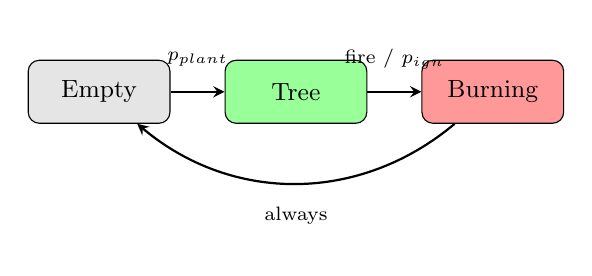
\begin{tikzpicture}[>=stealth, node distance=2.5cm, every node/.style={draw, rounded corners, minimum width=1.8cm, minimum height=0.8cm, font=\small}]
      \node[fill=black!10] (empty) {Empty};
      \node[fill=green!40, right of=empty] (tree) {Tree};
      \node[fill=red!40, right of=tree] (fire) {Burning};
      \draw[->, thick] (empty) -- node[above, draw=none, font=\scriptsize] {$p_{\text{plant}}$} (tree);
      \draw[->, thick] (tree) -- node[above, draw=none, font=\scriptsize] {fire / $p_{\text{ign}}$} (fire);
      \draw[->, thick, bend left=40] (fire) to node[below, draw=none, font=\scriptsize] {always} (empty);
    \end{tikzpicture}
  \end{center}
\end{frame}

\begin{frame}{Detecting Fire in the Neighbourhood}
  \begin{itemize}
    \item We use the \textbf{Moore neighbourhood} (8 surrounding cells).
    \item A helper function checks whether \textbf{any} neighbour has state 2 (burning).
  \end{itemize}
  \vfill
  \begin{center}
    \begin{tikzpicture}[scale=0.55]
      \fill[gray!20] (1,1) rectangle (4,4);
      \fill[green!60!black] (2,2) rectangle (3,3);
      \fill[red!80!black] (3,3) rectangle (4,4);
      \draw[gray] (0,0) grid (5,5);
      \node[font=\scriptsize] at (2.5, 2.5) {?};
      \draw[thick, primary] (1,1) rectangle (4,4);
    \end{tikzpicture}
  \end{center}
  \small
  The tree at the centre has a burning neighbour $\Rightarrow$ it will catch fire in the next step.
\end{frame}

\begin{frame}[fragile]{Updating a Single Cell}
  \begin{center}
  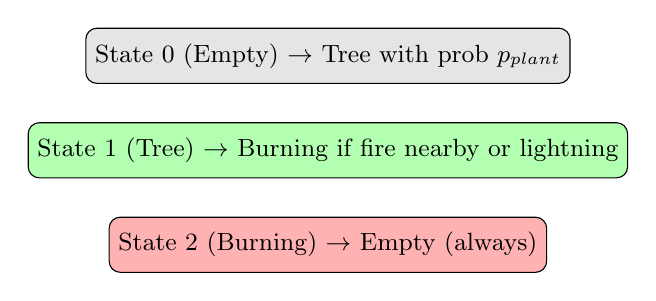
\begin{tikzpicture}[
    box/.style={draw, rounded corners, minimum width=5cm, minimum height=0.7cm, font=\small, text centered},
    >=stealth
  ]
    \node[box, fill=black!10] (e) at (0,0) {State 0 (Empty) $\to$ Tree with prob $p_{\text{plant}}$};
    \node[box, fill=green!30] (t) at (0,-1.2) {State 1 (Tree) $\to$ Burning if fire nearby or lightning};
    \node[box, fill=red!30]   (f) at (0,-2.4) {State 2 (Burning) $\to$ Empty (always)};
  \end{tikzpicture}
  \end{center}
  \vfill
  \begin{lstlisting}[escapechar=@]
def update_cell_state(state, fire_nearby,
                      p_plant, p_ignition):
    if state == 0:
        return 1 if random() < p_plant else 0
    if state == 1:
        if fire_nearby or random() < p_ignition:
            return 2
        return 1
    return 0  @\textcolor{neutral}{\# burning -> empty}@
  \end{lstlisting}
\end{frame}

\begin{frame}{Simulation Results}
  \begin{center}
    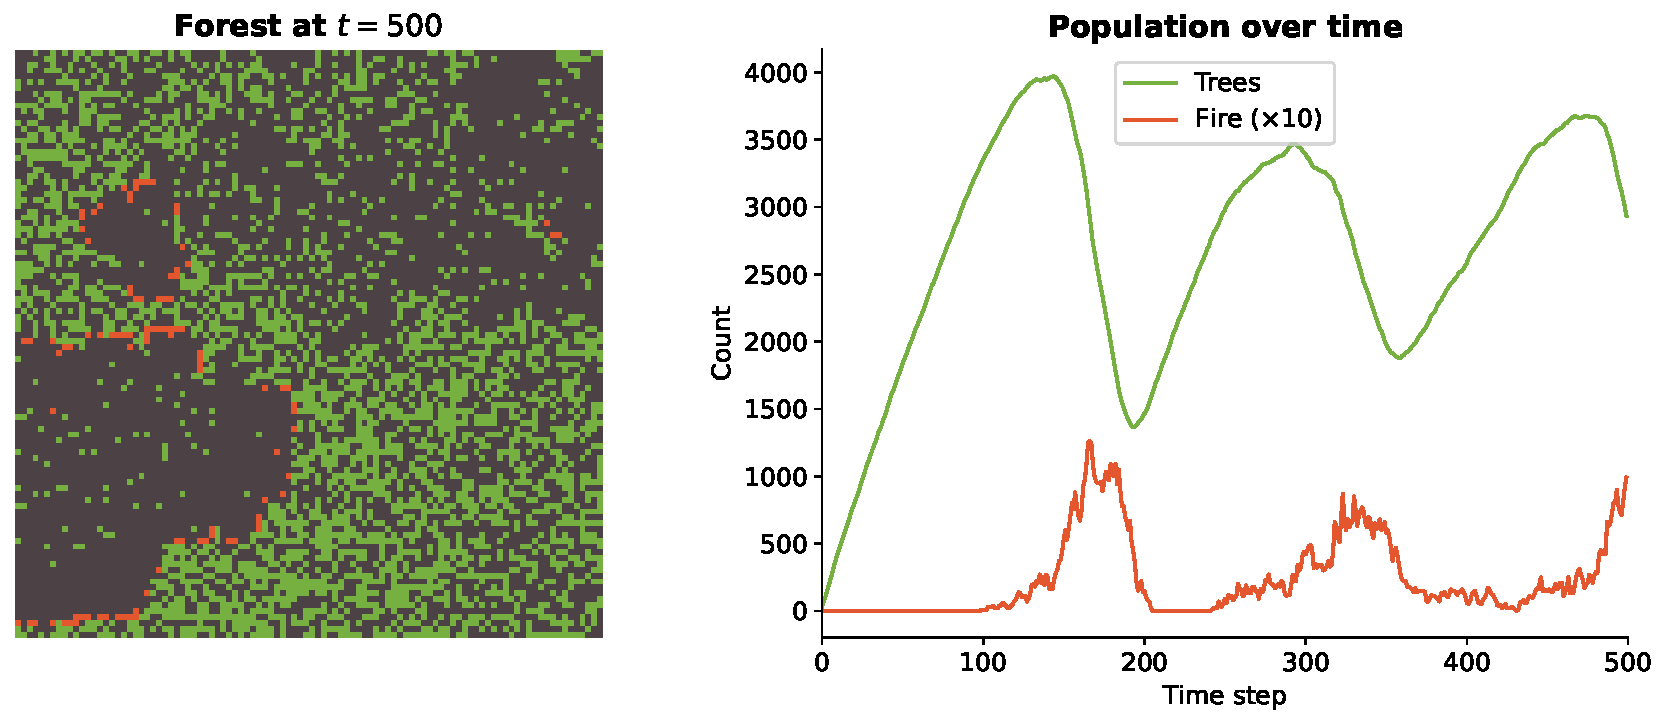
\includegraphics[width=0.9\textwidth]{images/forest_fire_simulation.pdf}
  \end{center}
  \small
  Left: spatial grid at a snapshot. Right: tree count and fire count over time.
  The system exhibits \textbf{self-organised criticality} --- large fires occur unpredictably.
\end{frame}

\begin{frame}{Self-Organised Criticality}
  \begin{itemize}
    \item Trees gradually fill the grid until a \textbf{critical density} is reached.
    \item A single lightning strike can then trigger a \textbf{large-scale fire}.
    \item After the fire, density drops and the cycle repeats.
    \pause
    \item This is an example of \textbf{self-organised criticality} (SOC):
    \begin{itemize}
      \item The system drives itself to a critical state without external tuning.
      \item Similar patterns appear in earthquakes, avalanches, and stock markets.
    \end{itemize}
    \item The distribution of fire sizes follows a \textbf{power law}.
  \end{itemize}
\end{frame}

\begin{frame}{Effect of Parameters}
  \begin{center}
    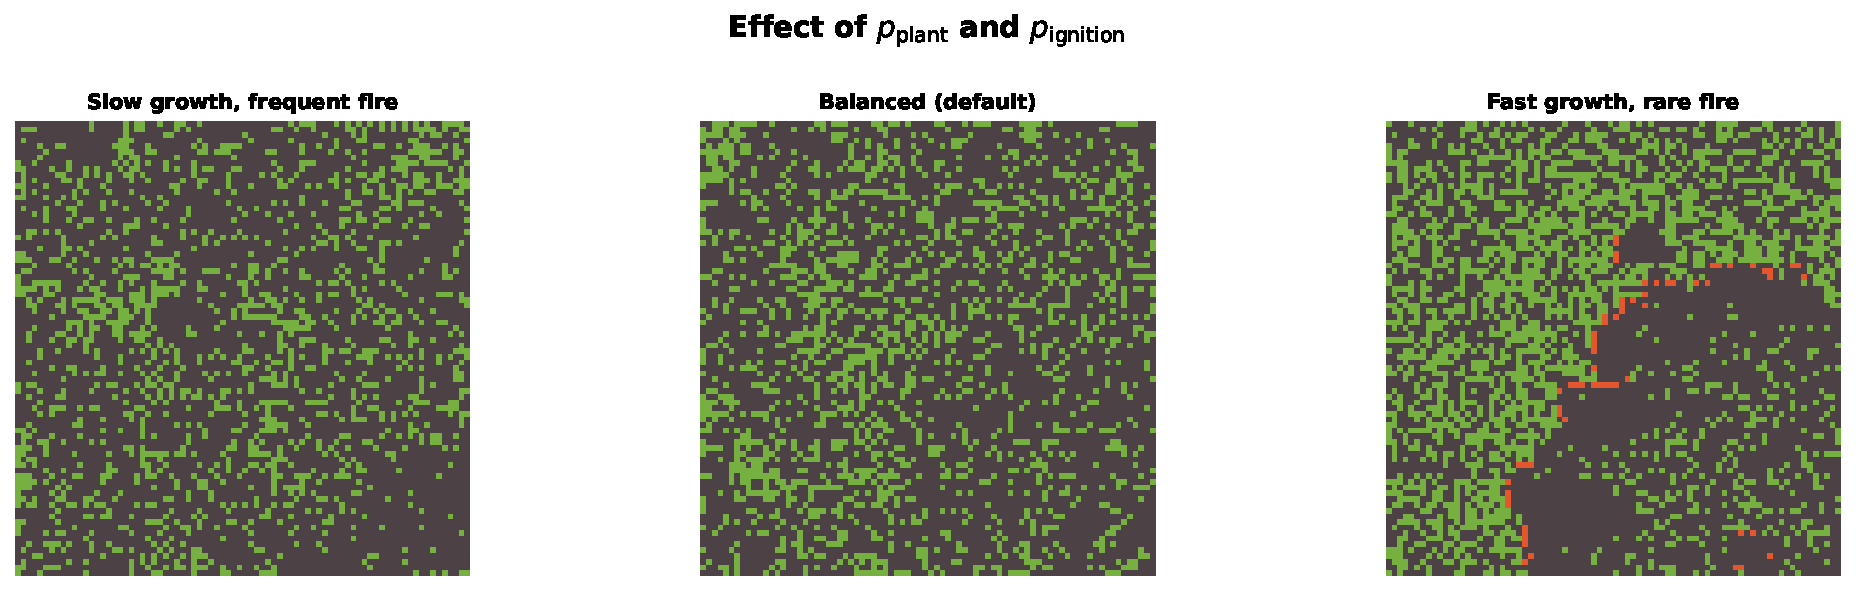
\includegraphics[width=0.9\textwidth]{images/forest_fire_parameters.pdf}
  \end{center}
  \small
  Varying the ratio $p_{\text{plant}} / p_{\text{ignition}}$ changes the frequency and size of fires.
\end{frame}

\begin{frame}{Exercise: Forest Fire}
  \begin{enumerate}
    \item Implement the \texttt{detect\_fire} function that checks for burning neighbours.
    \item Implement the \texttt{update\_cell\_state} function.
    \item Run the simulation and observe the dynamics.
    \item Experiment: what happens when you change $p_{\text{plant}}$ and $p_{\text{ignition}}$?
    \item Advanced: add \textbf{wind direction} --- fire spreads more easily downwind.
  \end{enumerate}
\end{frame}
